\documentclass{article} % Класс печатного документа

% для поддержки русского языка
\usepackage[T2A]{fontenc} % поддержка специальных русских символов
\usepackage[utf8]{inputenc} % Кодировка исходного текста - utf8
\usepackage[english,russian]{babel} % Поддержка языка - русского с английским
\usepackage{indentfirst} % Отступ в первом абзаце

\usepackage{hyperref} % Для вставки гиперссылок
% \usepackage{listings} % Для вставки кусков кода
\usepackage{graphicx} % Вставка изображений
\usepackage{subfig} % Изображения друг напротив друга
\usepackage{float} % Для точного позиционирования картинок

% Default fixed font does not support bold face
\DeclareFixedFont{\ttb}{T1}{txtt}{bx}{n}{12} % for bold
\DeclareFixedFont{\ttm}{T1}{txtt}{m}{n}{12}  % for normal

% Custom colors
\usepackage{color}
\definecolor{deepblue}{rgb}{0,0,0.5}
\definecolor{deepred}{rgb}{0.6,0,0}
\definecolor{deepgreen}{rgb}{0,0.5,0}

\usepackage{listings}

% Python style for highlighting
\newcommand\pythonstyle{\lstset{
    language=Python,
    basicstyle=\ttm,
    otherkeywords={self},             % Add keywords here
    keywordstyle=\color{deepblue},
    emph={MyClass,__init__},          % Custom highlighting
    emphstyle=\color{deepred},    % Custom highlighting style
    stringstyle=\color{deepgreen},
    frame=tb,                         % Any extra options here
    showstringspaces=false,           % 
    basicstyle=\small,                % уменьшить размер шрифта
    columns=flexible                  % чтобы при копировании не было пробелов везде
}}


% Python environment
\lstnewenvironment{python}[1][]
{
\pythonstyle
\lstset{#1}
}
{}

% Python for external files
\newcommand\pythonexternal[2][]{{
\pythonstyle
\lstinputlisting[#1]{#2}}}

% Python for inline
\newcommand\pythoninline[1]{{\pythonstyle\lstinline!#1!}}

\makeatletter
\def\lst@outputspace{{\ifx\lst@bkgcolor\empty\color{white}\else\lst@bkgcolor\fi\lst@visiblespace}}
\makeatother
 % для красивого оформаления python кода

\title{Отчёт 5\protect\\
    Классификация.\\
    Метод деревьев классификации и регрессии\\
    (classification and regression trees - cart)} % Заголовок документа
\author{Свичкарев А.\,В.} % Автор документа
\date{\today} % Текущая дата

\begin{document} % Конец преамбулы, начало текста

\maketitle % Печатает заголовок, список авторов и дату

\section{Цель}
Изучить способы решения задач классификации данных с
применением метода CART

\section{Задание №1}
Написать программу построения модели классификации данных методом CART и
визуализации дерева решений. Сравнить полное дерево с деревом, полученным после его
сокращения (pruning) с параметром 0.1.
\bigskip

Реализация взята из Приложения.
Но в исходном примере присутствует ошибка в функции вывода дерева в консоль.
\bigskip

Реализация алгоритма построения деревьев,
их вывода и предсказания (файл \verb$treeclassification.py$):
\pythonexternal{../treeclassification.py}

\clearpage
Запускающий модуль (файл \verb$exercise1.py$):
\pythonexternal{../exercise1.py}
\bigskip

Вывод программы:
\lstinputlisting{./ex1_output.txt}

\begin{figure}[H]
	\centering
	\subfloat[Оригинальное дерево]{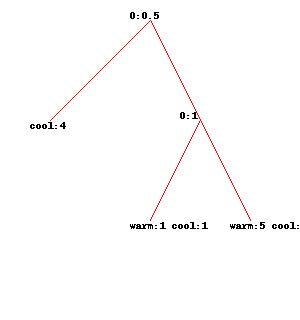
\includegraphics[width=0.5\textwidth]{./ex1_original_tree.jpg}}
	\hfill
	\subfloat[После сокращения]{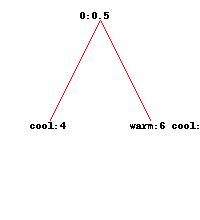
\includegraphics[width=0.5\textwidth]{./ex1_prune_tree.jpg}}
    \caption{Графические построения дерева}
\end{figure}

Видно, что после сокращения объединились ветки по первой ветви True.

\clearpage
\section{Задание №2}
Написать программу классификации тестовых данных в случаях полноты и
неполноты значений:
\bigskip

Запускающий модуль (файл \verb$exercise2.py$):
\pythonexternal{../exercise2.py}
\bigskip

Вывод программы:
\lstinputlisting{./ex2_output.txt}

\clearpage
\section{Задание №3}
Дополнить программу функцией кросс валидации (из предыдущей практической
работы) и оценить качество классификации данных из обучающей выборки.
\bigskip

Реализация функции кросс-валидации
и метрика оценки качества предсказания
по истинному классу и предсказанным классам в листе дерева
(файл \verb$crossvalidation.py$):
\pythonexternal{../crossvalidation.py}
Метрика возвращает 0,
если в листе находятся только классы истинного значения.
Метрика возвращает сумму остальных классов, если класс истинного значения
не входит в лист.
В остальных случаях метрика возвращает отношение числа класс истинного значения
в листе к сумме остальных классов.
\bigskip

Модуль оценки качества, запускающий кросс-валидацию (файл \verb$exercise3.py$):
\pythonexternal{../exercise3.py}
\bigskip

Вывод программы для соответствующих коэффициентов:
\lstinputlisting{./ex3_output.txt}

Чем больше итоговое значение, тем хуже дерево.
Однако если данных для обучения очень мало,
мы не может точно сказать,
ошибается ли дерево или у нас не достаточно просто сведений.
Поэтому с увеличением коэффициента валидации,
итоговые значения уменьшаются в среднем.

\section{Пояснение}
Исходный код доступен по ссылке:
\href{https://github.com/SvichkarevAnatoly/Course-Python-Bioinformatics/tree/master/semester2/task5}
{github.com}

\end{document} % Конец документа
